\documentclass{beamer}
\usepackage[ngerman]{babel}			%Deutsche Umlaute und Umbrüche
\usepackage[utf8]{inputenc}			%utf8 Kodierung
\usepackage{amsmath, amsfonts, amssymb, ulem} %Mathepackete schaden nie
\usetheme{Dresden}
\usecolortheme{beaver}
\usefonttheme{professionalfonts}
\title[WWWEKA]{World Wide WEKA}
\subtitle{Requirement Document}
\author[C. Heckmann\and C. Stricker\and D. Klopp\and M. Vieth]{Christian Heckmann\and Christian Stricker\and David Klopp\and Markus Vieth}
\date[\today]{\today}
\subject{Software engineering}
\newcommand{\btVFill}{\vskip0pt plus 1filll}
%Link zum Beamer-Userguid: ftp://ftp.dante.de/tex-archive/macros/latex/contrib/beamer/doc/beameruserguide.pdf
\begin{document}
	
	\frame{
		\titlepage
	}
	\setbeamertemplate{footline}[frame number]
	
	\frame[label=IV]{
		\frametitle{Inhaltsverzeichnis}
		\tableofcontents
		[pausesections]
	}
	
	\section[UR021]{Beispiel 1: User Requirement 021}
	\subsection[Statement]{Statement}
	\begin{frame}{Statement}{Browser}
		\begin{block}{UR021}
			"`Das System soll über alle gängigen Browser nutzbar sein (Desktop und Mobile): Firefox, Chrome, \sout{Opera,} Internet Explorer."'
		\end{block}
		\begin{alertblock}{Anmerkung:}
			Der Support von Opera wurde nach Absprache mit dem Übungsgruppenleiter gestrichen.
		\end{alertblock}
	\end{frame}
	
	\subsection[Resultierende Fragen]{Resultierende Fragen}
	\begin{frame}[<+->][t]{Resultierende Fragen}
		\begin{itemize}		
			\item Welche Browser werden aktuell verwendet?
			\item Werden alle Plattformen abgedeckt (Smart Device, Desktop)?
			\item Welche Browserversionen werden häufig eingesetzt?
			\item Werden die benötigten Funktionen unterstützt (HTML5, JavaScript)?
		\end{itemize}
	\end{frame}
	
	\subsection[Browser]{Browser}
	\begin{frame}[t]{Browserversionen}
		\begin{figure}
\centering
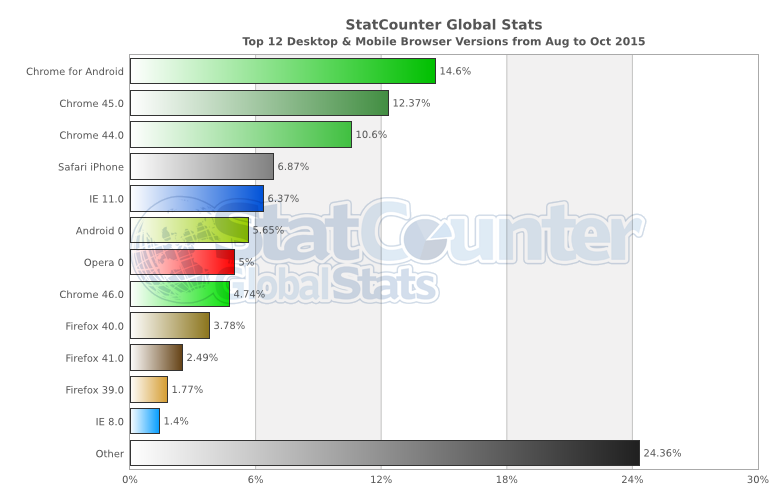
\includegraphics[width=0.85\linewidth]{./Bilder/StatCounter-browser_version-ww-monthly-201508-201510-bar}
\caption{gs.statcounter.com Browser Versionen}
\label{fig:StatCounter-browser_version-ww-monthly-201508-201510-bar}
\end{figure}

	\end{frame}
	\begin{frame}[t]{Browserversionen}
		\begin{columns}
				\column{.5\textwidth}
				\begin{description}	
				\item<1->[Google Chrome] 65,9\%
				\begin{description}
					\item<1->[4.7] 1,2\%
					\item<1->[4.6] 0,6\%
					\item<1-|alert@2>[4.5] 72,5\%
					\item<1->[4.4] 15,9\%
					\item<1->[4.3] 3\%
					\item<1->[4.2] 0,8\%
				\end{description}
			\end{description}
				\column{0.5\textwidth}
				\begin{description}
				\item<2->[Firefox] 20,6\%
					\begin{description}
						\item<2->[FF 42] 1\%
						\item<2->[FF 41] 9,2\%
						\item<2-|alert@2>[FF 40] 64,1\%
						\item<2->[FF 39] 5,3\%
						\item<2->[FF 38] 6,8\%
					\end{description}
				\end{description}
			\end{columns}
			\btVFill
			\onslide<2->{Quelle: w3schools.com}
		\end{frame}
		\begin{frame}
			\begin{columns}
				\column{0.5\textwidth}
				\begin{description}	
				
				\item<1->[Internet Explorer] 6,4\%
				\begin{description}
					\item<1-|alert@3>[IE 11] 65,6\%
					\item<1->[IE 10] 14\%
					\item<1->[IE 9] 14\%
					\item<1->[IE 8] 7,8\%
				\end{description}
				\end{description}
				\column{0.5\textwidth}
				\begin{description}
				\item<2-|alert@3>[Edge] 0,8\%
				\item<3-|alert@3>[Android Browser] 3,24\%
				\item<3-|alert@3>[MobileSafari] 1,21\%
			\end{description}
			\end{columns}
			\btVFill
			\onslide<3->{Quelle: w3schools.com}
	\end{frame}
	\begin{frame}[t]{HTML5}
			\begin{figure}
\centering
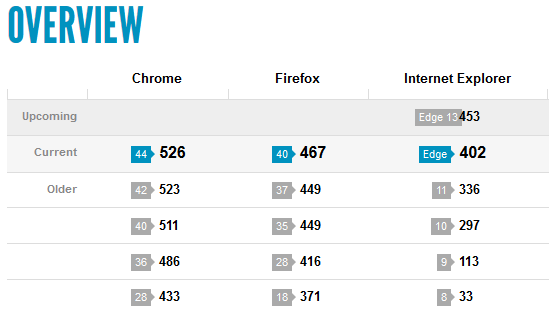
\includegraphics[width=0.93\linewidth]{Bilder/HTML5Desktop}
\caption{html5test.com Desktop}
\label{fig:HTML5Desktop}
\end{figure}
	\end{frame}
	\begin{frame}[t]{HTML5}
		\begin{figure}
			\centering
			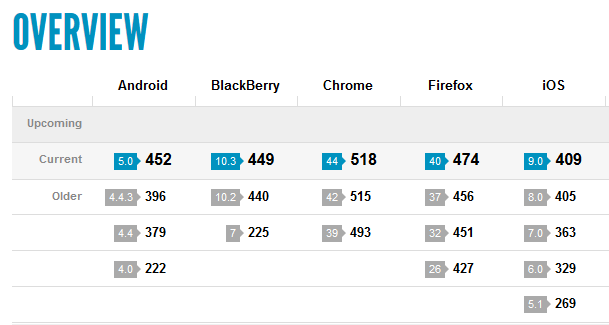
\includegraphics[width=1\linewidth]{Bilder/HTML5Mobile}
			\caption{html5test.com Smart Devices}
			\label{fig:HTML5Mobile}
		\end{figure}

	\end{frame}
	
	\section[UR003]{Beispiel 2: User Requirement 003}
	\subsection[Statement]{Statement}
	\begin{frame}{Statement}{Datenupload}
		\begin{block}{UR003}
			"`Nutzer sollen die benötigten Datensätze, Modelle, sowie Algorithmen von einem lokalen PC auf den Server hochladen können."'
		\end{block}
			
	\end{frame}
	
	\subsection[Resultierende Fragen]{Resultierende Fragen}
	\begin{frame}[<+->][t]{Resultierende Fragen}
		\begin{itemize}		
			\item Welche Formate werden unterstützt?
			\item Müssen die Daten überprüft werden?
			\item Was geschieht bei zu vielen gleichzeitigen Uploads?
			\item Was geschieht mit den Daten nach dem Upload ?
			\begin{itemize}	
				\item Wer hat Zugriff auf die Daten?
				\item Wie lange bleiben die Daten erhalten?
				\item Was gilt für den Gast Nutzer?
			\end{itemize}
		\end{itemize}
	\end{frame}
	
	\subsection[Upload Prozess]{Upload Prozess}
	\begin{frame}[<+->][t]{Upload Prozess}
		\begin{itemize}		
			\item Vor dem Upload:
			\begin{itemize}	
				\item Sichere Verbindung zwischen Client und Server (NFR021)
				\item Dateiformat prüfen (FR008)
				\item Dateigröße prüfen (NFR011)
			\end{itemize}
			
			\item Nach dem Upload:
			\begin{itemize}	
				\item Korrektheit der Daten (FR011)
				\item Algorithmus hochgeladen ? (NFR020)
				\item Verstoßen gegen bestehendes Recht (NFR031)
			\end{itemize}

			\item Speicherung der Daten:
			\begin{itemize}	
				\item In RDF Datenbank speichern (NFR027)
				\item Verfügbarkeit über REST-Protokoll (FR001, FR009)
				\item Dateiverwaltung (FR015)
				\item Download (FR027, 028)
			\end{itemize}
		\end{itemize}
	\end{frame}
		
\end{document}